\section{Problem Formulation}

With new innovations in satellite technology, from higher processing power to tactical data links capable of communicating with ground assets \cite{b10} to rapid deployment via reusable rockets, the potential for proliferated satellite networks 
capable of performing decentralized data fusion is becoming more realistic.
The case we will consider in this paper is a global coverage LEO satellite network with high processing power and communication capabilities. 
The goal of this network is to track ground targets of interest, doing all fusion, sensing, communication, and planning in the sky.

\subsection{The Fusion - Sensing Layer}

% talk about how this layer can help seperate or solve the typical DDF problem.

% How in this layer, talk about compute vs sensing etc. 

    % \begin{figure}[h]
    %     \centering
    %     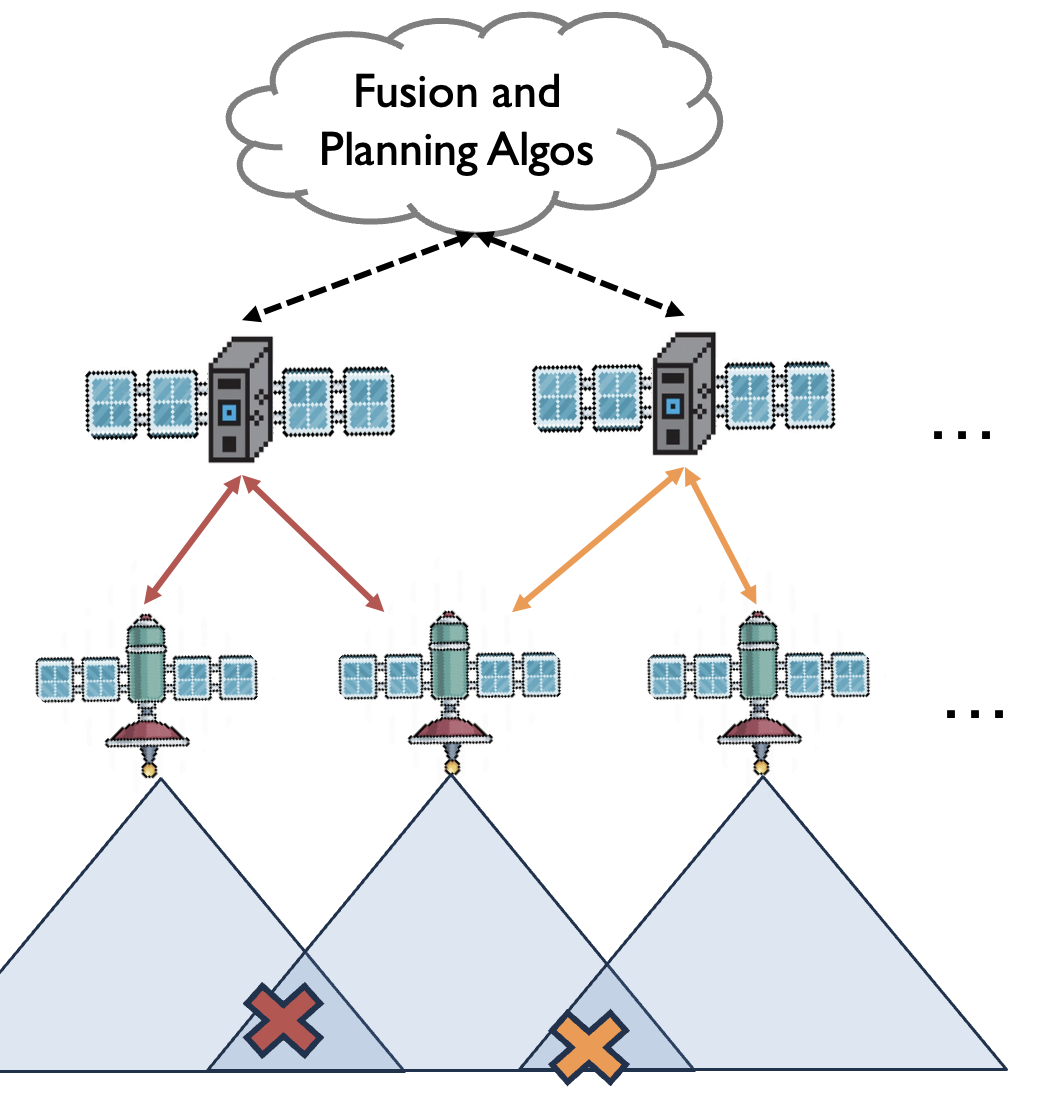
\includegraphics[width=0.35\textwidth]{figs/fusion_sensing_arch.png}
    %     \caption{Fusion - Sensing Architecture. The sensing layer is able to take measurements on targets (Xs) and communicate that back to the fusion layer. }
    %     \label{fig:satellite_structure}
    % \end{figure}

    The satellite network can be broken up into two layers of satellites; a sensing layer and a fusion layer. 
    The sensing layer consists of satellites that have powerful sensors capable of taking measurements on ground targets. 
    The fusion layer consists of satellites that have higher computational and communication capabilities allowing them to fuse measurements from the sensing layer. 

    The role of the sensing layer is to take measurements on ground targets. The sensing layer may contain a variety of sensors, 
    but, for simplification, we will assume all measurements taken are a bearings only measurement; a line of sight vector from a satellite to a predicted ground target.
    Once a sensing satellite has a measurement, it needs to communicate this measurement to the fusion layer for processing. 
    The fusion layer has the capability to recieve multiple measurements and generate an accurate track estimate using an Extended Kalman Filter. 
    The fusion nodes are also responsible for maintaining consistency in the track estimates. 
    This means that if two fusion nodes have conflicting track estimates, they must be reconciled using data fusion techniques such as covariance intersection, as mentioned in the background section.

\subsection{Federated Fusion}

% talk about how strcutred in a federated fusion approach. 

    \begin{figure}[h]
        \centering
        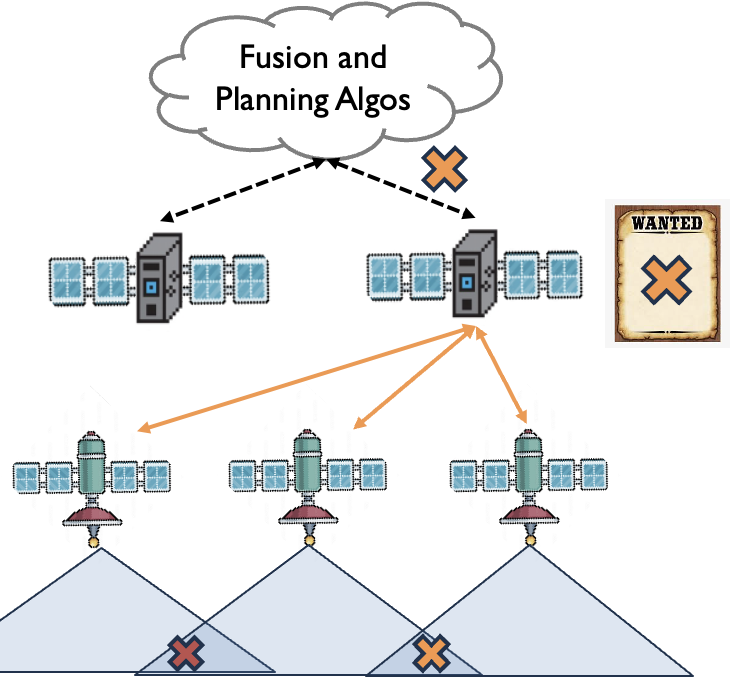
\includegraphics[width=0.35\textwidth]{figs/custody_bounty_sys.png}
        \caption{Federated Fusion Architecture. The fusion layer plans for custody, and assigns custody of the orange target to the right fusion node. This custody is then communicated to the sensing satellites. So that when those sensing satellites take a measurement on the orange target they send that to the fusion node that has custody of that target. }
        \label{fig:custody_bounty_sys}
    \end{figure}


    Federated fusion is a method of decentralized data fusion that allows for a dynamic programming type approach to data fusion.
    Instead of one centralized node being in charge of all tracks, sub-clusters of nodes can be assigned tasks.
    In the satellite tracking problem, federated fusion can be used to assign specific fusion nodes to be responsible for a specific track or region.
    If a fusion node is assigned a track, it will be the primary reciever of all measurements associated and will be responsible for the data fusion algorithms mentioned in the background section.
    Once a fusion node has been assigned "custody" of a track, all neccessary sensing satellites must be alerted of this. 
    Thus, when the sensing satellites take a measurement on that target or region, they know who to relay that data to in the fusion layer. 
    This entire process, which is called the "Custody-Bounty" system, is shown in Figure~\ref{fig:custody_bounty_sys} where the fusion nodes are shown with computers, the sensing satellites are shown with camera FOVs, and the targets are shown with Xs. 

    The key algorithm that is needed for this system to work is the ability to intelligently assign custody of targets to fusion nodes.
    Custody must be assigned while considering the computation constraints of the fusion nodes, each fusion node can only track a small number of targets due to computation limits.
    Additionally, communication limitations must also be considered. Satellites in a LEO constellation are able to communicate with eachother through a nearest neighbor communication network.
    Thus, if data needs to be sent a long distance in the network, it has to travel through multiple hops, which increases latency and bandwidth.
    
    The problem that will be addressed in this paper is how to assign custody of targets to fusion nodes while considering the computation and communication limitations of the system.
    
    % The communication links for a LEO satellite are limited, generally just neighbor to neighbor communication.
    % If communication has to travel further in the network, through multiple hops, latency will increase in the transmission, which impacts the performance of the fusion algorithms.
    % Thus, the problem that wille be addressed is how to assign custody of targets to fusion nodes while considering the computation and communication limitations of the system.


\subsection{Simulation Environment}

    To test the impact of federated fusion and optimization techniques, a Python simulation environment was created. 
    The class structure of this simulation environment is shown in Figure~\ref{fig:simulation_environment}.

    \begin{figure}[h]
        \centering
        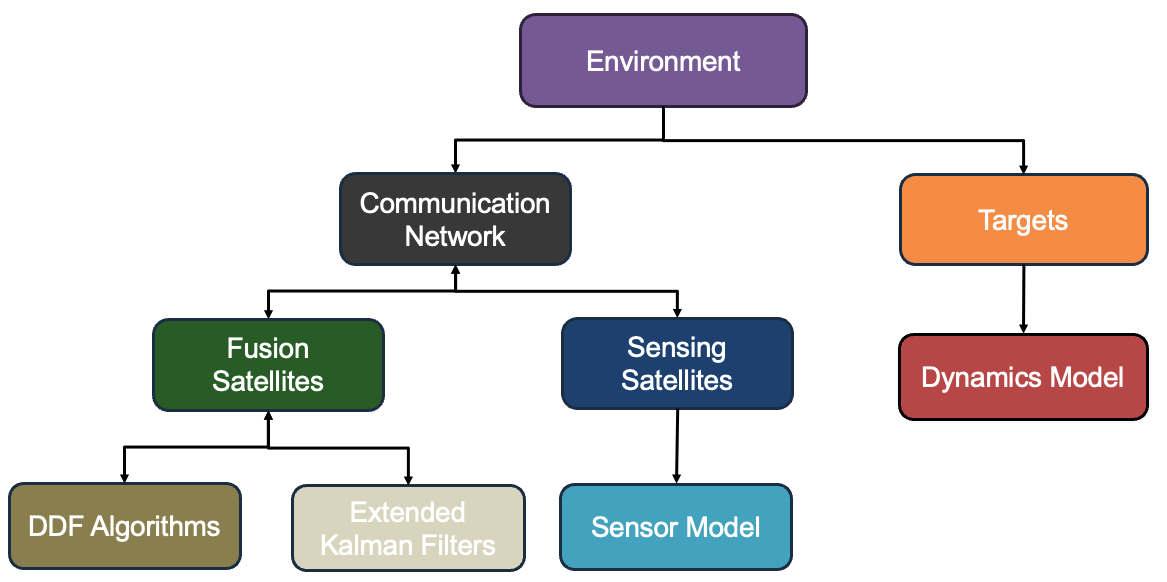
\includegraphics[width=0.45\textwidth]{figs/code_class_heirarchy.png}
        \caption{Simulation Environment Class Heirarchy}
        \label{fig:simulation_environment}
    \end{figure}

    This simulation environment is able to simulate scenarios with a large number of satellites and targets.
    All targets are given random spherical dynamics with speeds ranging from 0.3 to 5 Mach.
    Sensing satellites with sensors are able to take noisy measurements on these targets given by their sensor FOV and bearings errors.
    These measurements are then able to be sent through a realistic nearest neighbor communication network to fusion nodes.
    The fusion nodes are capable of taking batches of measurements and running extended kalman filters to generate track estimates. 
    Fusion nodes can also combine estimates from neighboring nodes using distrbuted data fusion (DDF) algorithms such as covariance intersection to generated a consistent track estimate.
    Assuming the fusion nodes are able to communicate in a centralized manner for planning, an algorithm can be used to assign custody of each estimated target to fusion nodes.
    Once custody is assigned, sensing satellites are given this information as a protocol of who to send their measurements to; allowing the federated fusion system to work.
    Thus, this simulation environment is capable of simulating a large variety of scenarios neccessary for the purpose of this paper, all future results and plots will be generated from this simulation environment.

    All code for this simulation environment is available via the GitHub link at the top of the paper.
    
